% Copyright (c) 2014,2016 Casper Ti. Vector
% Public domain.

\chapter{區塊鏈的實名交易監督系統與優化後系統實驗}

	\section{區塊鏈的實名交易監督系統實驗}
	根據比特幣點對點架構,儘管客戶和商店之間的交易細節已經快速存儲到雲數據庫,但官方確認交易與當前比特幣區塊鏈的交易通常需要更長的時間,因為需要確保確認的數量在交易廣播比特幣點對點網絡並存儲到緩存池後,是否存在雙重支付。
	因此,為了驗證我們提出的BRTMS不會通過使用比特幣等加密貨幣影響交易完成時間,我們在Testnet實驗中連續記錄了30筆交易信息。首先,我們使用區塊鏈工具,如\ref{fig9}的第一張快照所示,透過使用Testnet依序進行30筆比特幣交易,如圖\ref{fig9}的中間快照所示,最後30筆交易完成時間全部記錄在區塊鏈檢視器。實驗結果表明,實驗中的所有交易都在3秒鐘左右(平均2.97秒,標準差小於1秒)發送到比特幣網絡緩存池,平均交易完成時間在比特幣區塊鏈中確認為522.33秒(小於9分鐘),標準差大約為339秒。根據比特幣Testnet上的初步實驗結果顯示,我們提出的BRTMS可以快速有效地執行區塊鏈支付收款監督。

	\begin{figure}[h]
		\centering
		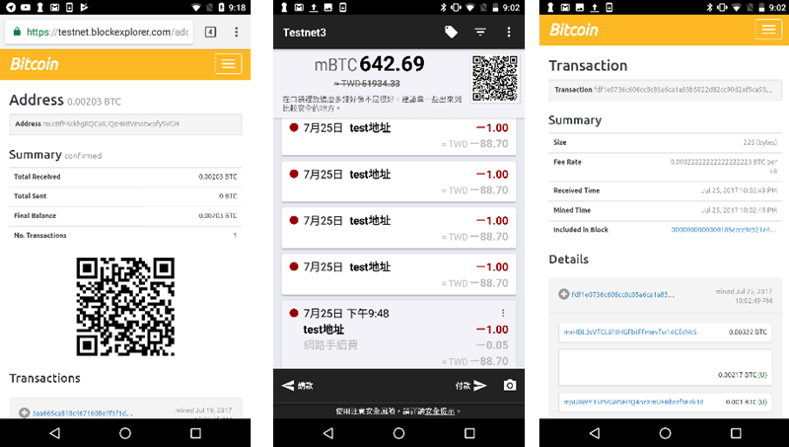
\includegraphics[width = 0.7\textwidth]{fig9.png}
		\caption{使用區塊鏈瀏覽器驗證存儲在比特幣區塊鏈中的交易過程}\label{fig9}
	\end{figure}

	\section{多重簽章優化區塊鏈的實名交易監督系統實驗}
		\subsection{交易效能實驗}
		本節主要介紹一般測試幣與Green Address錢包測試幣進行交易的效能實驗與結果分析,包含該實驗的目的、方法及結果分析。

			\paragraph{實驗目的}實驗的目的是要確認我們的系統在商家端進行行動支付時能快速、精準且高效率的進行交易,並瞭解使用一般Testnet錢包與Green Address錢包作為交易媒介的確認交易時間的差距。
			\paragraph{實驗方法}本次的實驗分為兩部份,分別是透過比特幣 Testnet錢包以及使用本論文所採用的Green Address 比特幣 錢包上執行25次付款,皆以相同地址收款,交易金額都設定為0.00001BTC, 實驗時間為2017年9月6日-17:00~17:50,每隔兩分鐘執行一次付款的動作,總共歷時50分鐘。兩款錢包同時發起交易,並透過區塊鏈檢視器進行記錄時間,最後再比較使用一般測試幣錢包及Green Address錢包兩者之間的差距。
			\paragraph{實驗結果}本次實驗分別記錄以Testnet錢包及Green Address錢包執行25次交易的進入緩存池等待時間和寫入區塊等待時間。若以Testnet錢包交易,必須等到交易寫入才能保證此筆交易不會被礦工遺棄,也才算真的完成這筆交易;但若以Green Address錢包發起交易就大不相同,當交易進入緩存池,即使遇到交易被礦工遺棄的情況,Green Address機構節點也會重新發起此筆交易,保證讓交易寫入區塊,所以只要進入緩存池我們就可以視為交易完成,透過兩者錢包的交易數據,我們比較及分析兩種錢包交易的時間數據。

%			\begin{figure}[h]
%				\centering
%				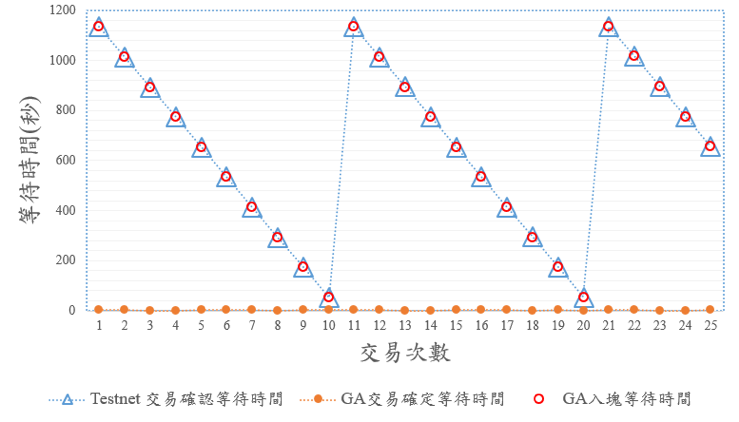
\includegraphics[width = 0.7\textwidth]{fig12.png}
%				\caption{fig12}\label{fig12}
%			\end{figure}

透過本次的實驗,我們可以發現雖然以兩種錢包交易進入區塊的等待時間完全相同,但因為Green Address錢包的特性,只要進入緩存池就算完成交易確認,因此Green Address錢包的完成交易確認的時間遠遠快於一般Testnet。相信以此⽅式作為主要⽀付管道,可以省去消費者在現金⽀付時掏零錢、算錢及找零等繁瑣的動作及時間,以此達成提升⽇常⽣活中的便利性與安全性。